\documentclass{article}
\usepackage[letterpaper, margin=25mm]{geometry}
\usepackage[parfill]{parskip}
\usepackage{tabularx}
\usepackage{graphicx}

\begin{document}
  \begin{titlepage}
    \begin{center}
      \vspace{4cm}
      \textbf{\huge Milestone 2} \\
      \textit{October 15, 2017} \\
      \vspace{1cm}
      Alqimlas, Naser \\
      Dinh, Matthew \\
      Hightower, Eleanor \\
      McMillan, Jon \\
      Shanks, William \\
    \end{center}
  \end{titlepage}

  \section*{Project Management Tool}
  Our team tracks our sprints and backlog in \textbf{Trello}. We integrate
  Trello with Github and Slack so that each service is syncing with the others. 

  \begin{center}
    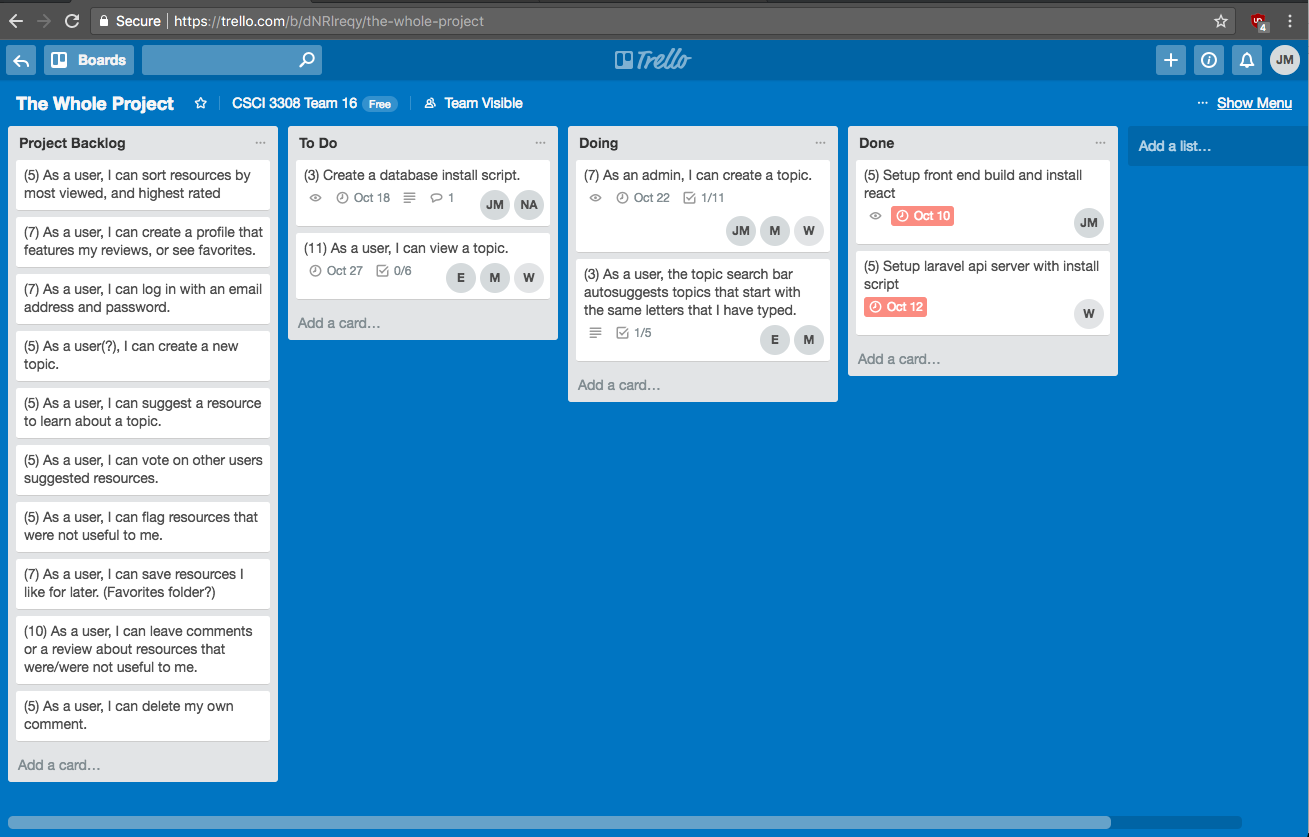
\includegraphics[width=10cm]{milestone_2_trello.png}
  \end{center}

  \section*{Plan Cycle}
  We will run 3 sprints with each sprint lasting 3 weeks. The final sprint will
  end just before the final presentations begin. We recognize that it will not
  be realistic to get through every desired feature in the 9 weeks. We will be
  sure that we follow the agile methodology and deliver fully functional
  features at the end of each sprint.  In this way we ensure there is a
  deliverable at the end of the course without committing to a particular set a
  features.

  \begin{center}
    \begin{tabular}{l|l|l}
      ~ & Start Date & End Date \\ \hline
      Sprint 1 & Monday, October 9 & Sunday, October 29 \\
      Sprint 2 & Monday, October 30 & Sunday, November 19 \\
      Sprint 3 & Monday, November 20 & Sunday, December 10
    \end{tabular}
  \end{center}

  \section*{Agile Methodology}
  Conclusions from our retrospective:
  \begin{itemize}
    \item It has been very difficult to arrange consistent meeting times to
      conduct them face-to-face.
    \item The very large difference in experience levels makes it difficult for
      members to contribute equally.
    \item The skills required to begin coding the project have not been taught
      yet.
  \end{itemize}
  \vspace{1cm}
  Things we will change to make it more productive:
  \begin{itemize}
    \item We will meet in smaller groups to share knowledge so more members can
      contribute effectively.
    \item We will give group members opportunities to specialize on parts of the
      project helping them to be more effective without overwhelming them with
      the large number of seperate tools and languages.
  \end{itemize}

\end{document}
